\documentclass[diss-proposta,nocipinfo]{texufpel}
%nocipinfo para não aparecer os dados da CIP no Resumo

\usepackage[utf8]{inputenc} % acentuacao
\usepackage{graphicx} % para inserir figuras
\usepackage[T1]{fontenc}

\hypersetup{
    hidelinks, % Remove coloração e caixas
    unicode=true,   %Permite acentuação no bookmark
    linktoc=all %Habilita link no nome e página do sumário
}

\unidade{Centro de Desenvolvimento Tecnológico}
\programa{Programa de Pós-Graduação em Computação}
\curso{Ciência da Computação}

\title{Estudo e Revisão das Técnicas de Mineração de Dados em Ambientes Educacionais}

\author{Costa}{Alexandre Gomes da}
\advisor[Prof.~Dr.]{Mattos}{Julio Carlos Balzano de}

%Palavras-chave em PT_BR
\keyword{mineração de dados educacionais}
\keyword{learning analytics}
\keyword{técnicas de predição}

%Palavras-chave em EN_US
\keywordeng{educational data mining}
\keywordeng{learning analytics}
\keywordeng{prediction techniques}

\begin{document}

\maketitle 
\sloppy

%Resumo em Portugues (no maximo 1 pagina)
\begin{abstract}
Uma grande quantidade de dados vem sendo produzida através de diversas modalidade de iteração em sistemas envolvendo alunos e professores. Contudo, grande parte desses dados não sofre qualquer tipos de analise. Nos últimos anos uma gama cada vez maior de trabalhos vem surgindo na área de Mineração de Dados Educacionais (MDE). Devido a essa grande quantidade de trabalhos é que se faz necessário fazer um levantamento para descobrir quais métodos, técnicas e algoritmos vem sendo utilizado, e ainda quais tipos de problemas vem sendo apurados. A pesquisa foi realizada, procurando responder as seguintes questões: Qual tem sido as técnicas utilizadas nos trabalhos na área. Qual tipo de dados estão sendo considerados pertinentes na área. Qual é o objetivo de estudo dos trabalhos na área. Qual são as ferramentas que tem sido utilizadas na área. O objetivo deste trabalho é fazer uma busca nas principais meios de publicações brasileiros que vem pesquisando MDE utilizando técnicas de predição.
\end{abstract}

\chapter{Motivação}
% (ENTRE 1 e 2 PÁGINAS)

% Nesta seção, apresenta-se um breve histórico da área de concentração
% da Dissertação, partindo do tema mais abrangente até chegar
% especificamente no assunto do Projeto. Além disso, apresenta-se a
% justificativa para a realização do trabalho, sua importância acadêmica
% ou para comunidade e grau de inovação. Poderá também apresentar as
% distinções entre o trabalho atual e outros trabalhos já realizados.

O uso constante de Tecnologia da Informação e Comunicação em diversas áreas vem gerando um grande volume de dados.
Tecnologias como a internet, redes sociais, ambientes virtuais de aprendizagem, dispositivo móveis, aplicativos embarcados, leitores de código de barras, sensores, leitores biométricos e sistemas de informação em geral são alguns exemplos de recursos que vem aumentando o numero de dados das mais diversas naturezas \cite{goldschmidt2015data}.

%% Educação
Atualmente, áreas como a educação produzem dados relacionados a alunos e professores todos os dias.
Necessidades da educação como sistemas para fazer o controle de iterações acadêmicas, gestão de projetos de pesquisa, ensino ou extensão, ou até mesmo sistemas para fazer o controle de gestão de pessoas são alguns do exemplos de sistemas que podem gerar um volume considerável de dados com frequência.

%% Knowledge Discovery in Database - KDD
Embora com ajuda de ferramentas computacionais, analisar essa crescente quantidade de dados não é trabalho para o homem \cite{goldschmidt2015data}. Para ajudar nesta questão a área de Descoberta de Conhecimento em Base de Dados (\textit{Knowledge Discovery in Database} - KDD) é focada em extrair conhecimento encima de granes volumes de dados. O termo mais conhecido relacionado a essa área é a Mineração de Dados (MD) que é uma das etapas do processo de KDD.

%% Mineração de dados educacionais
Segundo \citet{Koedinger2008} Mineração de Dados (MD) aplicada à educação é um campo interdisciplinar emergente mais conhecido como Mineração de Dados Educacionais (MDE).
\citet{baker2010data} define MDE como a área de investigação científica centrada no desenvolvimento de métodos para fazer descobertas dentro dos tipos de dados que vêm de ambientes educacionais e usando esses métodos para entender melhor os alunos e a aprendizagem deles. A Figura \ref{areas-relacionadas-mde} mostra que a área de MDE pode ser a combinação de 3 grandes áreas (ciência da computação, estatistia e educação) e serve de exemplo para justificar a interdisciplinaridade da área.

\begin{figure}[htbp]
  \centering 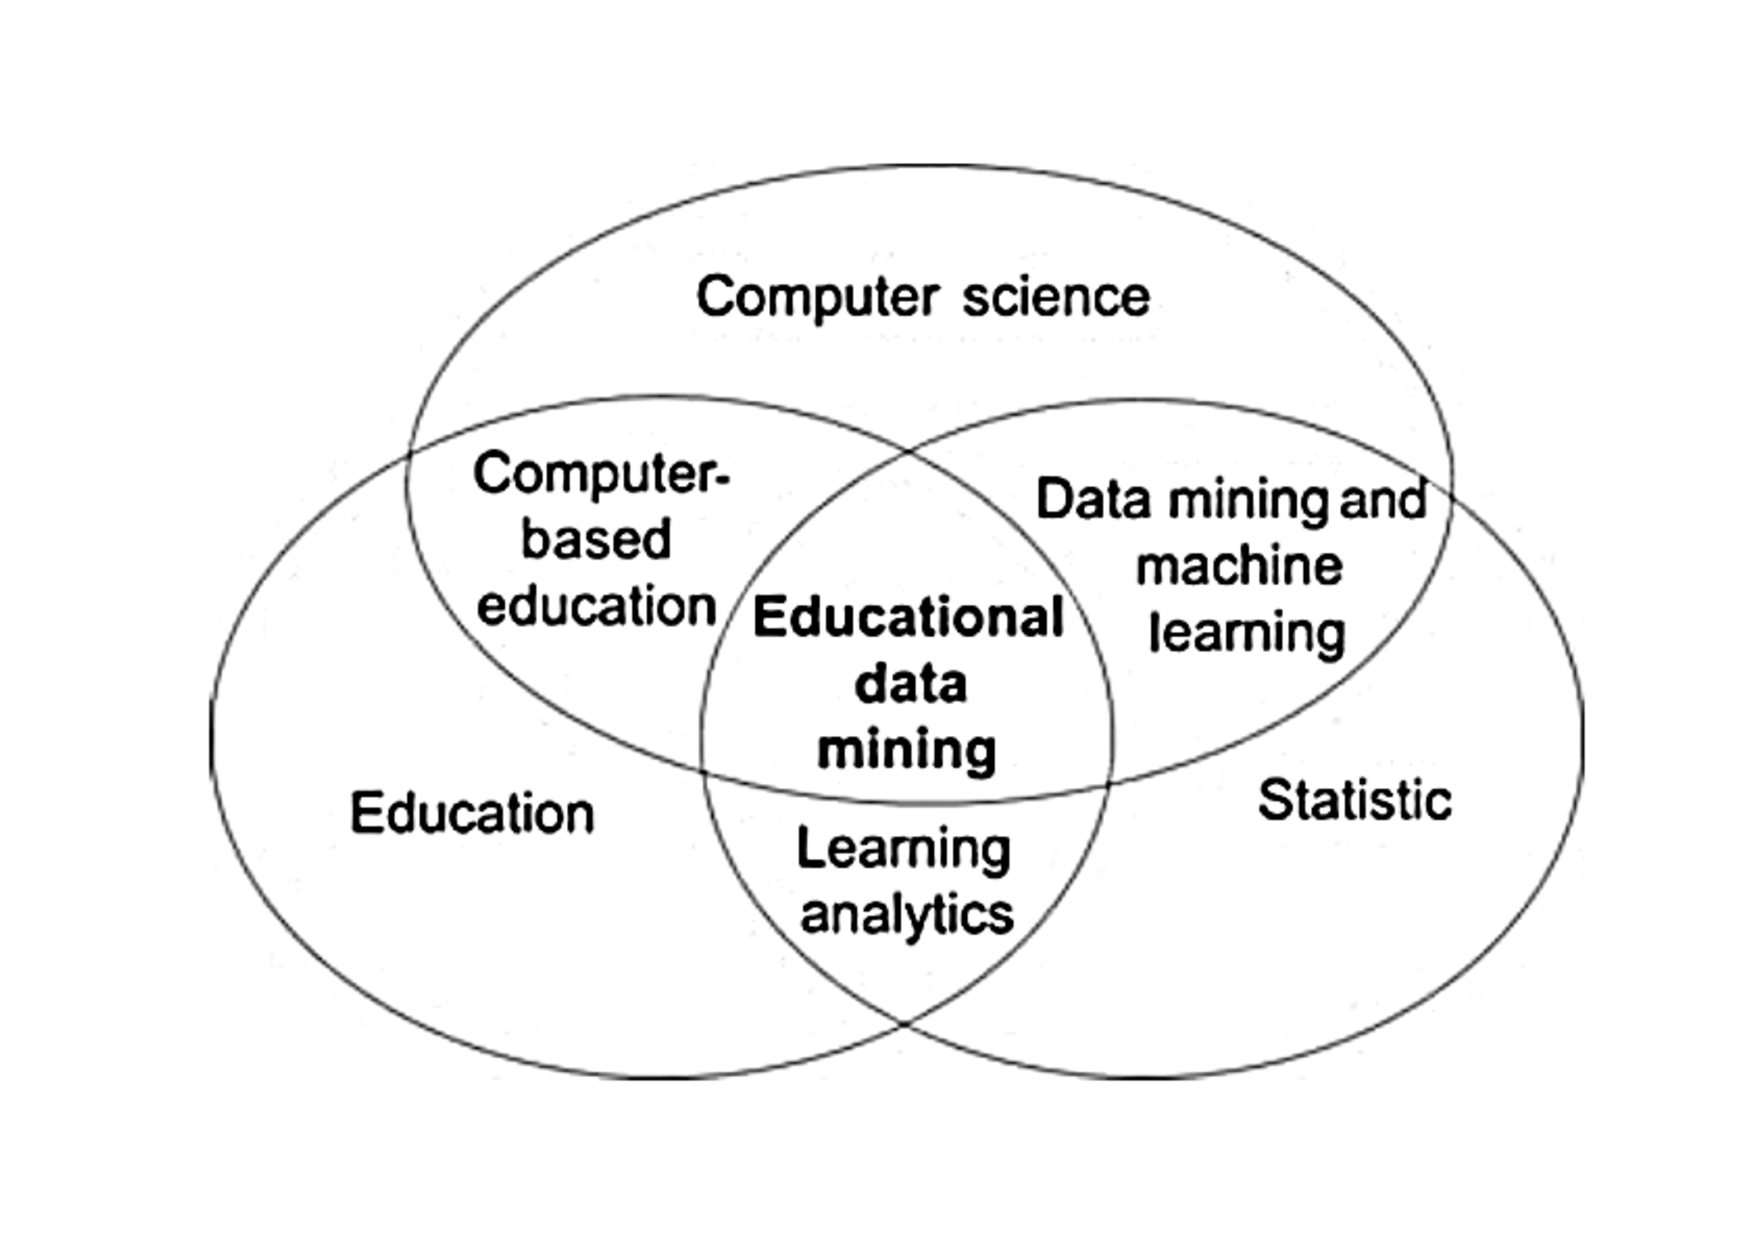
\includegraphics[scale=.4]{imagens/areas-edm.pdf}
  \caption{Principais áreas relacionadas com mineração de dados educacionais. \cite{Koedinger2008}}
  \label{areas-relacionadas-mde}
\end{figure}


%% Predição
Neste trabalho será aplicado um tarefa de classificação para tentar resolver o problema de evasão escolar. 
Segundo \citet{goldschmidt2015data} uma tarefa de classificação possui dois grupos. Um grupo contem normalmente um atributo apenas que vai servir para fazer a predição de um valor (atributo-alvo). Outro grupo corresponde aos atributos que vão servir para fazer a predição do valor (atributos de predição).
Tarefas de classificação são largamente utilizadas para fazer a predição de alunos em risco de evasão escolar, como será apresentado mais afrente.

\citet{baker2010data} agrupa o problema de evasão em uma categoria ou tarefa de detectar o comportamento do aluno.
Onde o objetivo é detectar os alunos que têm algum tipo de problema ou comportamento incomum, por exemplo: ações erradas, pouca motivação, trapaça, evasão escolar, etc.
Destaca também que as principais técnicas usadas para resolver esses tipos de problemas são de classificação e agrupamentos.

%% Justificativa
Este trabalho busca usar a base de dados do Cobalto que é o Sistema Integrado de Gestão da UFPEL. A base do Cobalto conta também com os dados históricos do GOL que foi o sistema acadêmico da UFPEL de 2006 à 2013. %% CONTINUAR

A grande vantagem deste estudo está na naturalidade dos dados. Quanto alguns trabalhos fazem questionários, provas, exercícios, etc, no presente trabalho serão coletado dados que foram gerados a partir de resultado que os alunos obtiveram em diversas disciplinas e cursos.

%% Importância acadêmica


%% Distinções entre o trabalho atual e os trabalhos já realizados

\chapter{Objetivos e Resultados}
% (ENTRE 1 e 3 PÁGINAS)

Este trabalho tem como objetivo estudar e aplicar técnicas de KDD aos dados do sistema Cobalto, para obter um padrão de predição da evasão de alunos através de dados inerentes aos estudantes da UFPEL. Para atingir este objetivo é preciso dividir o trabalho objetivos específicos.

O primeiro é investigar o que esta sendo pesquisado na área de mineração de dados educacionais, tentando focar em trabalho que tratam da evasão de alunos.

Em seguida é preciso fazer um levantamento do referencial teórico e apresentar os principais conceitos a repeito de mineração de dados educacionais. Mais especificamente seria estudar e apresentar os conceitos de KDD, mineração de dados e mineração de dados educacionais.

Por fim, criar e testar modelos de predição de alunos em risco de evasão de estudantes da UFPEL, utilizando os dados acadêmicos do aluno.

Em geral a grande maioria dos trabalho com este foco utilizam base de dados de sistemas de EAD. Neste trabalho será utilizado um base de dados histórica de alunos da UFPEL.

% Nesta seção, apresentam-se o objetivo Geral e os objetivos Específicos
% da dissertação. Os objetivos não devem ser confundidos com as
% atividades. Para a definição das atividades, deve-se partir dos
% objetivos determinados nesta seção. O objetivo Geral do Projeto
% necessariamente deve ser algum resultado prático (implementação) ou
% teórico (modelos formais ou especificações ou validações) produto da
% pesquisa realizada no período do Projeto. Assim como os objetivos
% específicos, que são considerados como sub-produtos do Objetivo
% Geral. Além disso, deve-se apresentar os principais resultados
% esperados do desenvolvimento desta dissertação.

\chapter{Metodologia}
% (ENTRE 1 e 3 PÁGINAS)

% O processo de mineração de dados envolve várias fases e etapas. Este trabalho classifica o processo de KDD em três grandes fases, com base nas abordagens descritas em [Silva and Vieira 2002] e [Rezende et al. 2003]: Preparação, Extração de Padrões e Pós-Processamento. Cada fase pode envolver uma ou mais etapas conforme mostra a tabela 1. No entanto, o KDD é um processo iterativo e algumas etapas podem ser realizadas novamente após a análise dos padrões encontrados de forma a melhorá-los \cite{Pimentel2006}.
O processo de descoberta de conhecimento envolve várias fases e etapas. Para o desenvolvimento deste trabalho será utilizada a abordagem proposta por [Silva and Vieira 2002] e [Rezende et al. 2003] onde o processo pode ser separado em três fases: Preparação, Extração de Padrões e Pós-Processamento. Cada fase pode envolver uma ou mais etapas. No entanto, KDD é um processo iterativo e algumas etapas podem ser realizadas novamente após a análise dos padrões encontrados de forma a melhorá-los \cite{Pimentel2006}.

Descoberta de conhecimento em base dados pode ser composto por várias etapas operacionais \cite{goldschmidt2015data}.
Este trabalho será dividido em 3 grandes momentos: coleta dos dados, pré-processamento dos dados, criar e avaliar os modelos de predição.

Na etapa de coleta será coletado todo o dado bruto referente aos alunos dos cursos de graduação da UFPEL. Esta etapa será feita de forma manual através de consultas a base de dados.
Os sistemas de aplicações, conhecidos por OLTP (On-Line Transaction Processing), processam dados armazenados em Base de Dados relacionais usadas para armazenar, consultar e alterar informações do negócio. Normalmente, não é possível aplicar as técnicas de MD diretamente a estas bases, pois isso poderia resultar numa sobrecarga de consultas nas mesmas podendo literalmente “travar” um sistema, impossibilitando qualquer outro tipo de operação transacional. 
Assim, é recomendável que os dados a serem utilizados na descoberta de conhecimento estejam separados da Base de Dados operacional. Nesses casos, utilização de DW é indicada, pois possibilita o armazenamento de grande quantidade de dados históricos de uma organização e viabiliza acessos otimizados aos dados previamente consolidados, reduzindo consideravelmente o tempo de realização do processo de MD \cite{Rezende2002}.

Em seguida vem a etapa de pré-processamento onde será verificado a necessidade de fazer a limpeza e classificação dos dados para serem utilizados nos testes. Da mesma forma que a primeira esta etapa também sera feita de forma manual.

De uma forma mais macro vem a terceira etapa onde será gerado um modelo de predição aplicando algoritmos de aprendizagem de máquina e posteriormente este modelo será avaliado a partir dos resultados.

O processo de mineração de dados envolve várias fases e etapas. Este trabalho classifica o processo de KDD em três grandes fases, com base nas abordagens descritas em [Silva and Vieira 2002] e [Rezende et al. 2003]: Preparação, Extração de Padrões e Pós-Processamento. Cada fase pode envolver uma ou mais etapas conforme mostra a tabela 1. No entanto, o KDD é um processo iterativo e algumas etapas podem ser realizadas novamente após a análise dos padrões encontrados de forma a melhorá-los \cite{Pimentel2006}.



% Nesta seção, apresenta-se a metodologia proposta para o
% desenvolvimento da Dissertação. O proponente deve descrever as
% atividades necessárias para a conclusão dos objetivos propostos. 

\chapter{Cronograma}

Esta seção deve apresentar relação numerada de atividades (de estudo,
modelagem, especificação, implementação ou validação) que deverão ser
realizadas (incluindo atividades obrigatórias como seminário de
andamento, entrega e apresentação da dissertação) e o cronograma
destas atividades, distribuídas no prazo de 12
meses.

\bibliography{bibliografia}
\bibliographystyle{abnt}

\chapter{Assinaturas}
\vspace{2cm}

\begin{center}
\rule{8cm}{.3mm}
\medskip

	Nome do Aluno\\
	Proponente

\end{center}

\vspace{4cm}

\begin{center}
\rule{8cm}{.3mm}
\medskip

	Nome do Professor\\
	Prof. Orientador

\end{center}
\end{document}
